% !TEX program = xelatex
\documentclass[UTF8,11pt,a4paper,fontset=fandol]{ctexart}

\usepackage[a4paper,top=2.15cm,bottom=2.25cm,left=2.25cm,right=2.25cm,headheight=15pt]{geometry}
\usepackage{setspace}
\usepackage{microtype}
\usepackage{booktabs}
\usepackage{tabularx}
\usepackage{array}
\usepackage{multirow}
\usepackage{makecell}
\usepackage{threeparttable}
\usepackage{amsmath,amssymb,mathtools}
\usepackage{newunicodechar}
\newunicodechar{≥}{\ensuremath{\geq}}
\usepackage{graphicx}
\usepackage{float}
\usepackage{subcaption}
\usepackage{xcolor}
\usepackage{enumitem}
\usepackage{listings}
\usepackage{algorithm}
\usepackage{algpseudocode}
\usepackage{fancyhdr}
\usepackage{titlesec}
\usepackage{hyperref}
\usepackage{xurl}
\usepackage{bookmark}
\usepackage[numbers,sort&compress]{natbib}
\usepackage[most]{tcolorbox}
\usepackage{tikz}
\usetikzlibrary{arrows.meta,positioning,shapes.geometric,fit,calc,backgrounds,matrix}

\definecolor{RPLBlue}{HTML}{285F9E}
\definecolor{RPLGreen}{HTML}{3F7F5F}
\definecolor{RPLOrange}{HTML}{CC7A29}
\definecolor{RPLRed}{HTML}{B94A48}
\definecolor{RPLGray}{HTML}{F3F5F7}
\definecolor{RPLDark}{HTML}{243447}

\hypersetup{
  colorlinks=true,
  linkcolor=RPLBlue,
  citecolor=RPLGreen,
  urlcolor=RPLOrange,
  pdftitle={RPLBench：面向工具调用智能体的冗余参数泄露评测数据构建},
  pdfauthor={赵嘉宁}
}

\graphicspath{{../figures/}}
\setstretch{1.22}
\setlength{\parindent}{2em}
\setlength{\parskip}{0.12em}
\setlist{nosep,leftmargin=2.2em}
\setcounter{secnumdepth}{3}
\setcounter{tocdepth}{2}
\emergencystretch=2em

\pagestyle{fancy}
\fancyhf{}
\fancyhead[L]{RPLBench：冗余参数泄露评测数据构建}
\fancyhead[R]{科研实习项目论文}
\fancyfoot[C]{\thepage}

\titleformat{\section}{\Large\bfseries\color{RPLDark}}{\thesection}{0.65em}{}
\titleformat{\subsection}{\large\bfseries\color{RPLDark}}{\thesubsection}{0.6em}{}
\titlespacing*{\section}{0pt}{1.8ex plus .4ex minus .2ex}{0.8ex}
\titlespacing*{\subsection}{0pt}{1.35ex plus .3ex minus .2ex}{0.5ex}

\newcolumntype{Y}{>{\raggedright\arraybackslash}X}
\newcolumntype{C}[1]{>{\centering\arraybackslash}p{#1}}
\newcolumntype{L}[1]{>{\raggedright\arraybackslash}p{#1}}

\newcommand{\RPL}{\textnormal{\textsc{RPL}}}
\newcommand{\RPLBench}{\textnormal{\textsc{RPLBench}}}
\newcommand{\ToolPrivacyBench}{\textnormal{\textsc{ToolPrivacyBench}}}
\newcommand{\code}[1]{\path{#1}}

\newtcolorbox{keybox}[1][]{
  enhanced,breakable,colback=RPLGray,colframe=RPLBlue,
  boxrule=0.7pt,arc=1.5mm,left=2mm,right=2mm,top=1.3mm,bottom=1.3mm,
  title=#1,fonttitle=\bfseries
}
\newtcolorbox{warningbox}[1][]{
  enhanced,breakable,colback=red!3,colframe=RPLRed,
  boxrule=0.7pt,arc=1.5mm,left=2mm,right=2mm,top=1.3mm,bottom=1.3mm,
  title=#1,fonttitle=\bfseries
}

\lstdefinestyle{rplcode}{
  basicstyle=\ttfamily\footnotesize,
  backgroundcolor=\color{RPLGray},
  frame=single,
  rulecolor=\color{gray!45},
  breaklines=true,
  showstringspaces=false,
  columns=fullflexible,
  keywordstyle=\color{RPLBlue}\bfseries,
  stringstyle=\color{RPLGreen},
  commentstyle=\color{gray}
}
\lstset{style=rplcode}

\title{\vspace{-1.5em}\textbf{RPLBench：面向工具调用智能体的\\[0.18em]冗余参数泄露评测数据构建}\\[0.35em]
\Large 基于 $\tau$-bench、BFCL、API-Bank 与 AppWorld 的可复现方法}
\author{赵嘉宁}
\date{2026年8月}

\begin{document}
\maketitle
\vspace{-1.5em}

\begin{abstract}
工具调用使智能体能够操作外部应用，也使用户信息随参数进入数据库、日志与第三方服务。现有评测主要考察工具选择、参数填写和任务完成情况，却较少区分"完成任务所必需的信息"与"工具虽然接受、但当前目的并不需要的信息"。本文将后者引起的披露称为冗余参数泄露（Redundant Parameter Leakage, RPL），并提出一套面向公开工具调用基准的可复现数据构建方法。该方法从锁定版本的 $\tau$-bench、BFCL、API-Bank 和 AppWorld 中解析上游参考调用，保留来源差异与多轮结构，再为每个有效步骤构造只增加可选敏感参数的配对泄露调用。最终数据包含 328 条任务，均通过结构校验、来源重放和执行检查，其中 321 条具有最终状态验证证据。本文以上游基准提供的参考调用作为功能参照，并采用统一的确定性规则生成参数权限标签，使构建结果可以复核和重复生成。该数据将冗余敏感信息披露与工具选择错误、必填参数缺失等一般调用错误区分开，为工具调用智能体的隐私评测提供了可执行、可追溯的实验样本。

\noindent\textbf{关键词：}工具调用智能体；隐私披露；数据最小化；冗余参数泄露；评测数据集；可复现研究
\end{abstract}

\section{引言}

智能体帮助用户取消一笔订单时，需要向订单系统传入订单编号。但如果它同时把用户的出生日期和支付卡号也填进了可选参数，订单一样能取消成功，敏感信息却已经发给了本不需要它的服务。这种披露既不是攻击者诱导的，也不影响任务完成——它只是智能体在拥有完整用户档案时，多传了几个字段。

本文将这种现象称为\textbf{冗余参数泄露}（Redundant Parameter Leakage, RPL）。它与提示注入攻击不同\citep{debenedetti2024agentdojo}：后者是外部攻击者试图改变智能体行为，前者发生在正常的、功能正确的任务执行中。它也不是参数填错——工具选对了、必填参数齐全、最终状态也正确，问题只是调用里多了几个本可删掉的敏感参数。

隐私研究早已指出，信息是否可以披露不能只看字段是否敏感，还要看它流向谁、为了什么目的\citep{nissenbaum2004contextual}。同一个电话号码，通知工具可能需要，但查询工具不需要。CONFAIDE 和 PrivacyLens 等工作进一步发现，模型嘴上说知道隐私规范，手上却可能照做不误\citep{mireshghallah2024confaide,shao2024privacylens}。\ToolPrivacyBench 把这一思路带进工具调用场景，发现任务完成率和隐私合规并不是一回事\citep{hu2026toolprivacybench}。AgentSCOPE 追踪信息在用户、智能体和工具之间的传播路径\citep{ngong2026agentscope}，Privacy in Action 关注动态工具生态中的判断与行动差距\citep{wang2025privacyinaction}。这些工作说明，只看最终回答或任务是否完成，不足以发现执行过程中的参数级泄露。

但要把现有工具调用任务改造成能评测 RPL 的数据，并不容易。$\tau$-bench、BFCL、API-Bank 和 AppWorld 四个基准各自保存参考调用的方式不同：有的是任务动作，有的是多轮对话，有的是逐条 API 记录，有的是通过环境验证的执行日志。它们对用户身份、工具可见范围和轨迹完整性的表达也不一样。如果转换时直接把这些记录都叫"标准答案"，不仅会丢掉来源信息，还可能把一条参考路径误当成唯一解或最短路径。

本文的做法是：不改变上游参考调用的任何参数，只在此基础上构造一个"多传了敏感字段"的对照版本。如图\ref{fig:rpl-motivation}所示，两条调用使用同一工具、同一必填参数，唯一区别是后者增加了若干可选的敏感字段。这样，隐私泄露就与工具选择错误、必填参数缺失等功能问题分离开来，差异精确落在多出来的参数上。

\begin{figure}[t]
  \centering
  \begin{tikzpicture}[
    font=\small,
    card/.style={rounded corners=2pt, draw, thick, align=left, inner sep=5pt},
    field/.style={font=\footnotesize, anchor=west},
    hdr/.style={font=\small\bfseries, anchor=west},
    arrow/.style={-{Latex[length=2mm]}, thick},
  ]
    % ---- 用户档案 ----
    \node[card, draw=RPLBlue, fill=RPLBlue!5, text width=4.2cm] (profile) {};
    \node[hdr] at ([xshift=5pt,yshift=-5pt]profile.north west) {用户档案};
    \node[field] at ([xshift=5pt,yshift=-20pt]profile.north west) {user\_id: sophia\_silva};
    \node[field] at ([xshift=5pt,yshift=-32pt]profile.north west) {email: s.silva@mail.com};
    \node[field] at ([xshift=5pt,yshift=-44pt]profile.north west) {date\_of\_birth: 1996-05-12};
    \node[field] at ([xshift=5pt,yshift=-56pt]profile.north west) {payment\_method\_id: cc\_7334};
    \node[field] at ([xshift=5pt,yshift=-68pt]profile.north west) {home\_address: 12 Oak St};

    % ---- 任务指令 ----
    \node[card, draw=RPLDark, fill=gray!6, text width=4.2cm, below=12mm of profile] (task) {};
    \node[hdr] at ([xshift=5pt,yshift=-5pt]task.north west) {任务};
    \node[field, text width=3.8cm] at ([xshift=5pt,yshift=-20pt]task.north west) {取消航班预订 IFOYYZ};

    % ---- Ground call ----
    \node[card, draw=RPLGreen, fill=RPLGreen!5, text width=4.6cm, below=10mm of task, xshift=-3.1cm] (ground) {};
    \node[hdr, text=RPLGreen] at ([xshift=5pt,yshift=-5pt]ground.north west) {不泄露调用};
    \node[field] at ([xshift=5pt,yshift=-20pt]ground.north west) {tool: cancel\_reservation};
    \node[field] at ([xshift=5pt,yshift=-32pt]ground.north west) {reservation\_id: IFOYYZ};

    % ---- Leaking call ----
    \node[card, draw=RPLRed, fill=RPLRed!4, text width=4.6cm, below=10mm of task, xshift=3.1cm] (leak) {};
    \node[hdr, text=RPLRed] at ([xshift=5pt,yshift=-5pt]leak.north west) {泄露调用};
    \node[field] at ([xshift=5pt,yshift=-20pt]leak.north west) {tool: cancel\_reservation};
    \node[field] at ([xshift=5pt,yshift=-32pt]leak.north west) {reservation\_id: IFOYYZ};
    \node[field, text=RPLRed] at ([xshift=5pt,yshift=-44pt]leak.north west) {+ date\_of\_birth: 1996-05-12};
    \node[field, text=RPLRed] at ([xshift=5pt,yshift=-56pt]leak.north west) {+ payment\_method\_id: cc\_7334};

    % ---- 结果 ----
    \node[card, draw=gray, fill=gray!4, text width=3.2cm, below=8mm of ground] (ok1) {};
    \node[hdr] at ([xshift=5pt,yshift=-5pt]ok1.north west) {结果};
    \node[field] at ([xshift=5pt,yshift=-20pt]ok1.north west) {预订已取消};

    \node[card, draw=gray, fill=gray!4, text width=3.2cm, below=8mm of leak] (ok2) {};
    \node[hdr] at ([xshift=5pt,yshift=-5pt]ok2.north west) {结果};
    \node[field] at ([xshift=5pt,yshift=-20pt]ok2.north west) {预订已取消};

    % ---- 箭头 ----
    \draw[arrow, RPLBlue] (profile) -- (task);
    \draw[arrow, RPLGreen] (task) -- node[left, font=\footnotesize] {必要参数} (ground);
    \draw[arrow, RPLRed] (task) -- node[right, font=\footnotesize] {+ 冗余参数} (leak);
    \draw[arrow, gray] (ground) -- (ok1);
    \draw[arrow, gray] (leak) -- (ok2);

    % ---- 标注 ----
    \node[font=\footnotesize\itshape, text=RPLRed, below=2mm of ok2, xshift=-1.55cm, text width=7cm, align=center]
      {RPL\_trigger\_params = \{date\_of\_birth, payment\_method\_id\}\\\textup{= keys(leaking) $-$ keys(ground)}};
  \end{tikzpicture}
  \caption{RPL 配对调用示例。不泄露调用只包含取消预订所需的 \texttt{reservation\_id}；泄露调用保留该参数不变，额外增加两个可选敏感字段。两次调用都成功取消预订，但后者向预订系统披露了不必要的出生日期和支付方式。触发参数精确等于两次调用的参数键差集。}
  \label{fig:rpl-motivation}
\end{figure}

围绕这一目标，本文回答三个问题：

\begin{enumerate}[label=\textbf{RQ\arabic*:}]
  \item 如何把四个结构各异的基准统一成同一套可审计的任务、工具、用户档案和调用表示，同时不丢失来源差异？
  \item 怎样保证每个泄露参数确实来自当前用户、在工具中是可选的、并且不影响原有调用？
  \item 如何区分"调用和源数据一致""调用能跑通""最终状态正确"这三种不同程度的验证，避免把一种证据当成完整证明？
\end{enumerate}

本文的主要贡献如下：

\begin{enumerate}
  \item 提出冗余参数泄露的配对构造方法：每步提供不泄露和泄露两个调用版本，差异只落在多出的可选敏感参数上，可以精确计算。
  \item 分析 $\tau$-bench、BFCL、API-Bank 与 AppWorld 的原始任务结构和验证机制，设计保留来源差异的适配与审计流程。
  \item 构建包含 328 条任务的 RPL 数据，逐条提供工具定义、用户档案、配对调用和来源证据。
  \item 分层报告结构校验、源重放、环境执行和最终状态验证的结果，并明确哪些是已验证的、哪些仍不是定论。
\end{enumerate}

本文不宣称已经获得人工业务授权意义上的最终标准答案，而是提供一个透明、保守、可重复运行的参数级隐私评测基础。下文依次介绍相关研究、源基准、数据构造、验证结果与局限。

\section{背景与相关工作}

\subsection{工具调用基准的演进}

工具调用评测已经从单次函数选择逐步扩展到多轮交互、环境状态变化和跨工具协作。早期的基准关注"智能体能否选对工具并填对参数"，随着智能体能力提升，评测焦点转向"能否在长程多步交互中可靠地完成任务"。本文使用的四个基准分别代表了这一演进的不同方向，它们为 RPL 研究提供了任务骨架，但都不直接评测隐私披露。

\subsubsection{$\tau$-bench：状态化多轮交互}

$\tau$-bench 针对的是已有基准的两个空白：它们只测单步、信息一次性给全的指令遵循，既没有人在回路的多轮交互，也不要求遵循领域特定策略\citep{yao2025taubench}。$\tau$-bench 以客服场景为切入点，让智能体在语言模型模拟的用户的动态对话中调用数据库 API，并遵守详细的策略文档。

$\tau$-bench 的奖励函数是二值的：动作正确性（最终数据库状态是否与标注一致）乘以输出正确性（回复是否包含用户所需信息）。在此基础上，它提出 pass$^k$ 指标衡量跨试验的一致性。两个领域各有特点：$\tau$-retail 处理订单取消、退换和地址修改，规则较简单；$\tau$-airline 涉及订票、改签和退款，策略更复杂且与会员等级和舱位挂钩，构成多跳推理难题。

$\tau$-bench 的用户档案包含 email、地址、支付方式和出生日期等字段，天然适合 RPL 研究。但其关键局限在于：奖励函数只比对最终数据库写状态，身份认证是读操作、不进入奖励，因此跳过认证也能获得满分，越权或跨用户泄露不会被惩罚\citep{yao2025taubench}。换言之，$\tau$-bench 测的是"把事做对"，而非"把事做得隐私合规"。

\subsubsection{BFCL：函数调用的综合评测}

BFCL 的动机是此前没有一个标准化的函数调用基准——判断一次调用是否"有效"本身很难，获取多样且真实的函数集合也不易\citep{patil2025bfcl}。BFCL 覆盖单轮（AST 匹配与真实执行）、多轮和智能体三类场景，跨 Python、Java、JavaScript 等多语言。

BFCL 的多轮数据定义为一个 query 序列与每轮期望的函数调用轨迹。它包含四个变体：base 是标准多轮任务；miss\_param 故意省略参数以测试追问能力；miss\_func 移除函数以测试澄清能力；long\_context 加长上下文以测试长程准确性。评测同时检查状态正确性（最终系统状态）和响应正确性（是否走了最小必要调用序列）。

BFCL 的局限与本文研究目标直接相关：它仅检查"调用是否正确"，不检查"调用是否该发生"。附录中仅提到"用户提示中的敏感信息被替换为占位符以保护隐私"\citep{patil2025bfcl}，但完全不考察模型是否应拒绝把敏感信息写进工具参数。其多轮 API codebase 是合成的模拟实现（如填油箱、查股价），不涉及真实企业级鉴权或数据最小化约束。

\subsubsection{API-Bank：工具检索与规划}

API-Bank 围绕三个递进能力构建：规划（plan）、检索（retrieve）和调用（call）\citep{li2023apibank}。它用"API 池大小"和"单轮调用次数"两个维度划分出三个 level：Level-1 评测已知 API 的参数填充，Level-2 要求先用 ToolSearcher 检索再调用，Level-3 要求自主规划并多步调用。评测集分别有 214、50 和 50 条对话。其 73 个 API 由工程师真实实现，涵盖天气、账号管理、日程、健康和财务等领域。

API-Bank 的对话大量涉及用户名、密码、token 和薪资等敏感信息，但论文未对工具调用链中的隐私风险做任何评测\citep{li2023apibank}。其伦理声明仅承诺访谈不泄露个人信息，未覆盖工具参数中的敏感数据处理。此外，Level-3 仅 50 条对话且复杂度有限，大部分对话是单步任务，多步推理能力远未被充分测试。

\subsubsection{AppWorld：可执行应用与状态测试}

AppWorld 认为已有基准只需 1--4 个 API 的线性调用，既不需要"富代码"也不需要智能体根据交互结果迭代改写代码\citep{trivedi2024appworld}。它构建了 9 个日常应用（Gmail、Venmo、Amazon、Spotify 等）的沙盒环境，包含 457 个 API 和约 37 万行底层数据库，让智能体完成跨应用的日常数字任务。

AppWorld 的评测采用基于最终数据库状态的程序化单元测试，而非逐条比对话步骤——因为复杂任务解法多样。它计算起始与结束数据库的 diff，断言期望的变更全部出现且没有附带损害（如任务没让退货却发起退货）。约 15\% 的任务是问答型，还需核对答案正确性。

AppWorld 的底层数据库是真实个人数字生活的镜像（邮件、转账记录、购物、联系人、支付卡），天然适合参数级隐私泄露评测。但其状态测试只关注任务目标和附带数据库改动，对"把不需要的敏感字段塞进可选参数"这类隐蔽泄露是盲区\citep{trivedi2024appworld}。此外，其官方 reference 调用序列只证明"任务可解"，不证明参数最小化或业务上必要。

\subsection{基于情境和用途的隐私判断}

隐私风险不能仅由字段是否敏感决定。上下文完整性理论指出，信息传递是否适当取决于信息主体、发送者、接收者、信息类型和传递原则\citep{nissenbaum2004contextual}。CONFAIDE 将这一理论用于语言模型的信息分享判断\citep{mireshghallah2024confaide}；PrivacyLens 则在行动场景中评估语言模型对隐私规范的理解，并表明模型的口头判断与实际行动可能不一致\citep{shao2024privacylens}。NIST 和 OECD 的隐私框架同样强调目的限制与数据最小化\citep{nist2017privacyengineering,nist2020privacyframework,oecd2013privacy}。

在工具调用场景中，同一信息对不同工具可能具有不同必要性。支付方式对支付工具是必要信息，但对商品查询工具并非必要；电话号码对通知工具可能必要，但不应进入内部分析备注。因此，本文把隐私标签定义为"某项具体用户信息对某个工具是否为完成当前步骤所必需"，而不是给字段分配一个全局允许或禁止状态。

\subsection{ToolPrivacyBench 与本文的关系}

\ToolPrivacyBench 首次将用途限制引入工具调用智能体的隐私审计\citep{hu2026toolprivacybench}。它把隐私泄露建模为知识库审计问题：每个 case 包含用户任务、工具集、私有原子集和字段-工具授权矩阵，智能体在 mock 后端执行后，审计器检测其工具参数中是否包含 forbidden 的私有原子。其 MT-POI 指标聚合多个子指标（字段机会归一化过披露率、严重度加权率等），在 9 个主流智能体上发现任务完成率高达 92--98\% 但 MT-POI 仍达 19--28，证明任务成功与隐私合规是两个独立维度。

\ToolPrivacyBench 的公开派生数据使用与本文相同的四个上游基准作为工作流骨架，并采用相同的筛选门槛（至少四次源调用、两个不同工具、四个敏感原子和二十个 forbidden 机会）。但其数据构造方式与本文有三个本质区别：

第一，\ToolPrivacyBench 的隐私泄露是\emph{被动观察}智能体执行行为得到的——它依赖智能体在 mock 后端执行时主动把多余信息写入参数或自由文本字段。本文则\emph{主动构造}配对调用：每一步保留上游 reference 作为不泄露参照，并构造一个仅在可选参数中增加敏感字段的泄露参照。这使得泄露是确定性的、可复现的，且与智能体行为无关。

第二，\ToolPrivacyBench 的授权标注采用 tool-purpose-first 的人工加规则方式，并对 215 个抽样 case 做了双人一致性验证（Cohen's $\kappa$ = 0.84--0.88）。本文采用确定性的 reference-argument matching 启发式规则，明确声明这不是人工业务授权金标准。

第三，\ToolPrivacyBench 关注自由文本字段（message、note、summary）中的泄露，并专门设计了 FreeTextFOR 等指标。本文聚焦 optional 结构化参数，每个泄露参数精确对应一个 entity 字段，避免把多个敏感原子塞入通用文本字段。

本文不复现 \ToolPrivacyBench 的后端模型实验，也不使用其人工一致性结果。当前工作定位为数据集构建研究，重点在于如何从四个锁定来源稳定地生成可审计的 RPL 契约，而非比较不同智能体的隐私表现。

\subsection{与智能体安全研究的区别}

RPL 属于正常任务中的非对抗性过度披露，不假设攻击者篡改提示、工具或环境。AgentDojo 等工作主要研究提示注入如何诱导智能体执行恶意动作或泄露信息\citep{debenedetti2024agentdojo}。两类问题都需要观察工具调用轨迹，但威胁模型不同：提示注入关注攻击是否改变行为，本文关注在正常任务中是否披露了超出当前用途的信息。RPL 不需要攻击者存在——只要智能体拥有完整用户档案且工具接受可选参数，过度披露就可能自然发生。

\section{源基准及其适配依据}

本文选择 $\tau$-bench、BFCL、API-Bank 和 AppWorld，是因为它们分别覆盖用户交互、通用函数调用、工具检索与跨应用执行等典型任务形态，且都提供了可追溯的调用证据。但这些证据在原论文中的含义并不相同：有的保存目标动作，有的保存多轮参考调用，有的记录单次 API 请求—结果，有的由最终状态评测器判定任务。本节先回到各基准的任务设计和数据结构，再说明本文从中继承了什么、不能据此声称什么。

\subsection{\texorpdfstring{$\tau$-bench}{tau-bench}}

\subsubsection{任务结构与评测机制}

$\tau$-bench 面向航空和零售客服场景\citep{yao2025taubench}。每个任务由用户指令和一组参考动作（actions）组成：用户指令是一段自然语言，描述用户想完成什么（如取消预订、交换商品、修改地址）；原论文中的 actions 主要包含达到目标状态所需的数据库写操作和需要向用户传达的输出信息，读取操作允许智能体自行决定。零售域有 115 条任务，航空域有 50 条，共 165 条。

任务环境包含结构化数据库：用户档案（email、地址、支付方式、出生日期）、订单、商品、航班和预订记录。智能体在与模拟用户的多轮对话中调用工具，必须遵守退款、改签、身份核验等业务规则。评测不逐字匹配固定轨迹，而是比较执行后的数据库状态是否与标注一致，并结合任务要求检查最终回复是否包含用户所需信息。论文采用 pass$^k$ 衡量重复试验中的稳定成功率。

\subsubsection{适配依据}

本文锁定版本的 \code{tasks\_test.py} 提供了比原论文标注更完整的 typed reference sequence：其中不仅包含写操作，还包含查询（如 \code{get\_user\_details}、\code{get\_reservation\_details}）、搜索（如 \code{search\_direct\_flight}）和计算（如 \code{calculate}）等中间步骤。本文将这些读、写和计算步骤统一作为源参考动作，通过源重放和环境状态检查确认可用性。由于原评测允许智能体通过不同交互过程达到目标状态，这些动作不能自动解释为唯一或最短解，本文不追加最小性声明。

$\tau$-bench 的用户、订单和支付方式都保存在结构化数据库中，用户身份可以由任务标识和数据库记录交叉核对，适合提取用户档案。同时，原生执行揭示出 16 条源参考序列包含业务错误（如查询不存在的商品、对非已交付订单执行换货）。本文没有修补这些序列，而是将其保守过滤。

\subsection{BFCL}

\subsubsection{任务结构与评测机制}

BFCL 是一个综合性函数调用基准，覆盖单轮、并行、多语言和多轮场景\citep{patil2025bfcl}。其多轮部分围绕八组状态化 API（交易、旅行、文件系统、消息、工单等）构造任务，每条任务包含一个多轮查询序列和对应的参考调用轨迹。多轮数据有四个变体：base 是标准多轮任务；miss\_param 故意省略参数以测试追问能力；miss\_func 移除函数以测试澄清能力；long\_context 加长上下文以测试长程准确性。

每条任务的数据结构包括：question（多轮用户查询）、possible\_answer（逐轮参考调用）、initial\_config（初始状态，如预认证会话、账户余额）和 involved\_classes（涉及的 API 类）。评测同时使用 state-based checker 检查最终系统状态是否匹配，以及 response-based checker 检查产生请求结果所必需的调用路径——后者尤其用于无法通过状态变化判断的只读任务。这不等价于对整条参考轨迹进行全局最小性证明。

\subsubsection{适配依据}

本文使用 200 条 base 多轮任务。possible\_answer 保存逐轮参考调用，initial\_config 提供可恢复的初始状态。对于会修改状态的任务，其他调用顺序可能同样正确；对于查询型任务，响应检查会对必要步骤提出更强约束。本文保留原有轮次边界和参考顺序，将其称为"源参考调用"，不把 possible\_answer 解释为经过全量消融的最短 Gold。

BFCL 的主要适配挑战是语义对齐：相同字符串可能在不同 API 类中表示密码、访问令牌、股票代码或普通文本，用户指令中的身份也可能与某个默认 profile 冲突。本文只接受能够由 API 类、参数名、初始状态和指令身份共同支持的字段映射；不能确定时放弃该字段或过滤任务。

\subsection{API-Bank}

\subsubsection{任务结构与评测机制}

API-Bank 将工具调用能力分为三个递进层级\citep{li2023apibank}。Level-1（直接调用）给定 API 定义，评测模型能否按查询正确填参调用，本质是参数填充。Level-2（检索后调用）API 未知且数量大，模型须先用 ToolSearcher 按关键词检索相关 API，再调用单个 API。Level-3（规划—检索—调用）要求模型自主规划并多步调用，难度最高。评测集分别有 214、50 和 50 条对话。

其 73 个 API 由工程师真实实现，涵盖天气、账号管理、日程、健康和财务等领域。对话以多轮形式组织，每个 AI 回合可能产出 API 请求，系统执行后回填结果。每条 API 记录保存请求参数（param\_dict）和返回结果（result），ToolSearcher 是一个特殊 API，输入关键词后返回最相关 API 的元信息。

评测方式为：初始化 API 数据库后，比较预测调用与人工标注调用是否产生相同查询或修改，并检查返回结果是否一致。API 调用使用 Accuracy 评价，调用后的自然语言回复使用 ROUGE-L 评价。这是一种逐调用的一致性检查，而非 AppWorld 那种整段任务的最终状态 evaluator。

\subsubsection{适配依据}

本文使用 214 条 Level-1 对话和 50 条 Level-2 对话，共 264 条源记录。Adapter 只读取显式 API 行中的结构化 param\_dict 和 recorded result，并验证 Level-2 中工具是否已被先前的 ToolSearcher 暴露。Level-3 样例没有与上述两层相同的结构化执行契约，因此没有与其混合。

这里的参考证据粒度是"单次 API 请求—结果"。将同一对话中的多次 API 行连接为一个调用序列，是本文为形成统一评测样本所作的适配，而非 API-Bank 原论文提供的对话级最终状态证明。由此产生的 7 条发布任务可以证明请求记录与上游一致、调用可执行，但不声称具有与 AppWorld 相同强度的最终数据库 oracle。

\subsection{AppWorld}

\subsubsection{任务结构与评测机制}

AppWorld 构建了 9 个日常应用（Gmail、Venmo、Amazon、Spotify、SimpleNote、Splitwise、Todoist、Phone、FileSystem）的沙盒环境，包含 457 个 API、101 张数据库表和约 37 万条数据库记录\citep{trivedi2024appworld}。底层数据由 106 名虚构人物和程序化生成的活动数据填充，模拟虚构人物数字生活的合成数据库。任务让智能体完成跨应用的日常数字任务，如"根据 SimpleNote 里的健身计划播放一个时长够今天锻炼的 Spotify 歌单"。

每条任务包含：任务指令、任务专属数据库副本、期望终态值和评测程序。评测采用基于最终数据库状态的程序化单元测试：计算执行前后的数据库 diff，断言期望的变更全部出现且没有附带损害（如任务没让退货却发起退货）。约 15\% 的任务是问答型，还需核对答案正确性。任务分为 train（105）、dev（60）、test\_normal（168）和 test\_challenge（417）四个 split。

\subsubsection{适配依据}

本文使用 147 条同时具备任务、方案 API 日志（ground\_truth/api\_calls.json）和可执行验证条件的记录，全部来自 dev 和 train split。test\_normal 和 test\_challenge 的任务没有 api\_calls.json，只有 answer.json 和 evaluation.py，不提供标准调用序列。上游 validation solution 的作用是证明任务可解并为数据生成提供参考执行，论文并未把它定义为规范路径或参数最小性证明。

AppWorld 的状态评测能够判断任务目标和数据库副作用，却不直接判断某个已传递参数是否符合当前用途。本文因此另行构造参数级配对调用；其中敏感 optional 参数属于本文的合成扩展，而非 AppWorld 原生接口。

\subsection{证据分层与统一表示}

表\ref{tab:source-characteristics}从任务结构、可见信息、状态环境、参考证据和原始评测五个维度比较四个基准。四个来源最终都会转化为统一调用对象，但统一表示不改变原始证据角色。

\begin{table}[t]
  \centering
  \caption{四个源基准的任务结构与评测机制比较。}
  \label{tab:source-characteristics}
  \scriptsize
  \begin{tabularx}{\textwidth}{L{1.4cm}L{1.6cm}L{1.8cm}L{1.6cm}L{1.8cm}Y}
    \toprule
    来源 & 任务单元 & 智能体可见信息 & 状态环境 & 参考证据 & 原始评测 \\
    \midrule
    $\tau$-bench & 用户模拟任务 & 工具、领域政策、对话 & 航空/零售数据库 & 动作与输出标注 & 数据库状态 + 传达信息 \\
    BFCL & 多轮用户查询 & 函数文档、历史轮次 & 八类状态化 API & \code{possible\_answer} & state + response checker \\
    API-Bank & API 对话 & API 描述或 ToolSearcher & API 数据库与结果 & 人工 API records & 调用一致性 + ROUGE-L \\
    AppWorld & 跨应用数字任务 & ApiDocs、Supervisor、执行历史 & 可重置应用数据库 & validation solution log & DB diff 程序化测试 \\
    \bottomrule
  \end{tabularx}
\end{table}

这种区分直接决定了本文的验证口径。来源重放回答"输出调用是否仍与锁定来源一致"；环境执行回答"调用能否在相应实现中运行"；最终状态验证回答"运行结果是否满足来源任务的状态判据"。三种证据可以同时存在，也可以只具备前两种，任何一种都不自动证明参数已经达到业务意义上的最小集合。

\section{源调用的适配与统一表示}

四个源基准对任务、工具和参考调用的保存方式差异很大。$\tau$-bench 把任务写成 Python 构造器，BFCL 将多轮问题与参考答案分置于两组 JSONL，API-Bank 把一次对话拆成 User、AI 和 API 记录，AppWorld 则保存 HTTP 级方案执行日志。如果直接在这些文件上编写隐私构造逻辑，同一项检查会出现四套实现，来源语义也容易在格式转换中丢失。本文因此把数据构建分为两个阶段：Adapter 只负责恢复上游事实，公共 Builder 再负责档案、授权、筛选与配对调用生成。

\subsection{Adapter 的职责边界}

Adapter 是一个确定性的源格式解析器。它接收锁定的 benchmark 目录，输出一组内部任务对象及解析统计；其职责包括定位正式数据文件、恢复工具 schema、解析参考调用、确定当前任务可见的工具，并保存能够解释这些结果的来源路径。Adapter 不读取隐私字段配置，不计算 allowed/forbidden，不选择泄露步骤，也不根据调用数或敏感字段数筛选任务。由此，同一份 Adapter 输出可以在不重新解释上游数据的前提下供不同构造策略复用。

源版本检查位于 Adapter 之后、Builder 之前。系统根据 Adapter 声明的完整输入文件集合，核对源仓库 revision 与逐文件哈希。该顺序很重要：输入锁覆盖 Adapter 实际读取的文件，而不是预先假定的一组目录；新增或遗漏输入都会改变锁定结果。通过检查后，后续流程只接收已经绑定来源版本的任务对象。

\begin{figure}[t]
  \centering
  \begin{tikzpicture}[
    font=\small,
    box/.style={rounded corners=2pt, draw, thick, align=center, inner sep=5pt, minimum height=9mm},
    source/.style={box, draw=RPLBlue, fill=RPLBlue!5, text width=3.0cm},
    adapter/.style={box, draw=RPLGreen, fill=RPLGreen!6, text width=2.6cm},
    common/.style={box, draw=RPLOrange, fill=RPLOrange!7, text width=3.0cm},
    audit/.style={box, draw=gray, fill=gray!8, text width=3.0cm, font=\footnotesize},
    arrow/.style={-{Latex[length=2mm]}, thick},
  ]
    \node[source] (files) {锁定的源文件\\\footnotesize 任务·工具·状态·参考调用};
    \node[adapter, right=10mm of files] (adapter) {Source Adapter\\\footnotesize 解析与规范化};
    \node[common, right=10mm of adapter] (case) {\code{SourceCase}\\\footnotesize calls·tools·state·provenance};
    \node[common, right=10mm of case] (builder) {公共 Builder\\\footnotesize 筛选·授权·配对构造};
    \node[audit, below=9mm of adapter] (lock) {\code{SOURCE_LOCK.json}\\revision + input hashes};
    \node[audit, below=9mm of case] (contract) {Source contract\\origin + role + visibility};
    \draw[arrow] (files) -- (adapter);
    \draw[arrow] (adapter) -- (case);
    \draw[arrow] (case) -- (builder);
    \draw[arrow, dashed] (files) -- (lock);
    \draw[arrow, dashed] (adapter) -- (lock);
    \draw[arrow, dashed] (adapter) -- (contract);
    \draw[arrow, dashed] (contract) -- (case);
  \end{tikzpicture}
  \caption{Adapter 边界。上游文件先被解析为保留来源语义的 \texttt{SourceCase}，通过版本锁定后才进入公共构造流程；隐私规则不进入 Adapter。}
  \label{fig:adapter-boundary}
\end{figure}

\subsection{统一内部对象}

对任务 $c$，Adapter 输出

\begin{equation}
S_c=(d_c,x_c,C_c,T_c,U_c,M_c),
\end{equation}

其中 $d_c$ 是来源内的任务域，$x_c$ 是用户指令，$C_c=(a_1,\ldots,a_n)$ 是按来源顺序恢复的参考调用，$T_c$ 是该任务可见的工具集合，$U_c$ 是可用于恢复用户或环境状态的结构化数据，$M_c$ 保存文件、索引和来源角色等追溯信息。调用 $a_i=(t_i,g_i)$ 由规范工具名 $t_i$ 和参数映射 $g_i$ 组成。

代码中的 \code{SourceCase}、\code{SourceTrace}、\code{NormalizedCall} 和 \code{NormalizedTool} 分别承载这些信息。表\ref{tab:adapter-interface}列出公共 Builder 实际依赖的字段。这里的”统一”仅指访问接口一致。

\begin{table}[t]
  \centering
  \caption{Adapter 的统一输出接口及其保真要求。}
  \label{tab:adapter-interface}
  \small
  \begin{tabularx}{\textwidth}{L{3.1cm}L{3.2cm}Y}
    \toprule
    字段 & 内容 & 必须保持的性质 \\
    \midrule
    \code{source\_case\_id} & 上游任务标识或稳定派生标识 & 能唯一回到来源任务，不使用发布序号替代 \\
    \code{instruction} & 来源任务中的用户需求 & 仅做空白规范化，不补写任务意图 \\
    \code{trace.calls} & 规范工具名与参数映射 & 工具、参数值和调用顺序与来源记录一致 \\
    \code{trace.origin/role} & 调用来自何处、承担何种证据角色 & 区分目标动作、参考调用、聚合记录与执行日志 \\
    \code{turn\_boundaries} & 扁平调用序列中的轮次结束位置 & 有多轮结构时保留；来源未提供时写为 null \\
    \code{tools} & 当前任务可见的工具 schema & required、类型、返回值和可见范围可验证 \\
    \code{source\_state} & 用户档案或环境初态中的可用事实 & 不把无连接依据的局部身份合并为同一用户 \\
    \code{provenance} & 文件、split、行号、哈希或任务目录 & 足以复查每项适配决策 \\
    \bottomrule
  \end{tabularx}
\end{table}

统一对象在进入 Builder 前满足四项基本条件。第一，每个调用都能在 $T_c$ 中找到唯一 schema；第二，调用参数覆盖全部 required 参数并通过类型检查；第三，存在轮次边界时，边界单调不减且最后一个边界等于调用数；第四，\code{origin}、\code{role}、工具可见性依据和来源检查项均为非空的显式值。违反这些条件的任务在 Adapter 阶段拒绝，而不是带着不完整信息进入隐私构造。

\subsection{四类来源的规范化方法}

\subsubsection{$\tau$-bench：受限 AST 解析}

$\tau$-bench 的正式任务和工具定义是 Python 源码。Adapter 使用 \code{ast.parse} 检查 \code{Task(...)}、\code{Action(...)} 和工具 \code{get\_info()} 的语法树，只对预期节点调用字面量求值，不导入上游模块，也不执行其中的任意代码。每个 action 的名称必须属于当前领域工具表，参数必须符合工具声明。airline 与 retail 可能出现同名工具，因此规范名增加领域前缀，例如 \code{airline\_\_cancel\_reservation}。

任务去重键为 $(domain,user\_id,instruction)$。键相同且 actions 完全一致的记录折叠；同键但 actions 冲突的记录整体拒绝，避免由文件遍历顺序决定保留哪条轨迹。用户状态从对应领域的 \code{users.json} 读取。若参考调用显式指向唯一且不同的 \code{user\_id}，实体身份以调用目标为准，并在 provenance 中同时保存任务身份与解析后的实体身份；如果一条任务指向多个用户，则 Adapter 直接报错。

\subsubsection{BFCL：多轮边界与函数类作用域}

BFCL 以任务 ID 连接 question 和 possible answer。两侧 ID 集必须完全相同，重复 ID 或单侧缺失都会使转换失败。\code{possible\_answer.ground\_truth} 是按轮组织的函数调用字符串；Adapter 使用表达式模式的 AST 解析函数名、位置参数和关键字参数，不允许字典展开、未知参数或重复赋值。解析后的调用被扁平化，同时记录每一轮结束时的累计调用数，因此公共 Builder 可以顺序处理调用，又不会丢失原始轮次。

工具可见范围由 \code{involved\_classes} 决定。Adapter 只合并这些函数类的文档；若两个可见类对同名函数给出不同 schema，该名称被标记为歧义，不参与静默覆盖。\code{initial\_config} 原样进入 source state，供后续环境恢复和档案构造使用。它描述整个任务的初态，而不是某个单独轮次的输入。

\subsubsection{API-Bank：请求—结果绑定}

API-Bank 的工具 schema 从 \code{apis/} 下的 Python class 静态恢复。Adapter 读取类级 \code{description}、\code{input\_parameters} 和 \code{output\_parameters}，并根据 \code{call()} 函数签名区分必填参数。对话只接受角色为 User、AI 或 API 的 JSONL 行，其中只有显式 API 行进入参考调用。文件名和 AI 自然语言回复均不用于猜测工具调用。

每条 API 行必须同时给出 \code{param\_dict} 和 recorded \code{result}。安全类型规范化后，请求参数应与 \code{result.input} 的键和值一致，\code{result.exception} 必须为空，且参数仍需通过原生 schema。Level-2 还维护 ToolSearcher 已暴露工具集合：除 ToolSearcher 本身外，后续调用只有在之前的搜索结果中出现过才被接受。同一对话的 API 行按原顺序聚合为 $C_c$，User 行则确定 turn boundaries；原始请求和结果的摘要写入 provenance，便于检查聚合是否改变记录。

\subsubsection{AppWorld：HTTP 日志到工具调用}

AppWorld 的方案日志记录 HTTP method、URL 和 request data，而工具文档使用带占位符的 path template。Adapter 以 method 与路径模板进行唯一匹配，将 URL 中的路径参数按 schema 恢复为整数、数值、布尔值或字符串，再与 request data 合并。找不到路由、匹配多个路由或合并参数不符合 schema 时，任务均被拒绝。

当前任务可见工具取 \code{required\_apis.json} 与方案日志实际调用工具的并集。指令与任务用户来自 \code{specs.json}，private/public task data 进入 source state，并保留各自来源。\code{ground\_truth/api\_calls.json} 提供的是上游方案执行日志；Adapter 只恢复调用，不在转换阶段启动 AppWorld。独立环境执行及最终状态判断在评测阶段进行，避免把“日志成功解析”误写成“本项目已经执行”。

\subsection{SourceRules 与来源契约}

格式差异由 Adapter 处理，构造政策差异则集中在 \code{SourceRules}。每个来源注册一份契约，声明参考调用的 origin、role、可见工具依据、应出现的来源检查项以及是否包含轮次边界。Builder 在渲染报告时写入这些声明，Validator 再与注册值逐项比较，因此修改 Adapter 的解释口径会成为可检测的协议变化。

\code{SourceRules} 还提供三类来源专属函数：选择档案模板、从结构化状态提取字段，以及把工具归类为 internal、service provider、bank 或 public audience。与解析相关的事实留在 Adapter，与隐私构造相关的政策留在 SourceRules，二者没有通过大量条件分支混入公共 Builder。

\subsection{保守失败与 Reference 完整性}

适配阶段采用拒绝优先的策略。无法唯一确定工具、参数与 schema 不一致、来源身份冲突或请求—结果无法绑定时，不修写 reference，也不根据常识补齐调用。另有一类问题只能在原生环境中发现，例如工具返回“商品不存在”或业务状态不允许当前操作。这些任务仍可由 Adapter 忠实解析，但发布政策根据锁定的执行证据将其排除，并在 conversion report 中逐条记录 case ID 和原始错误。

发布链在参考序列前增加一次 \code{LoadEntityProfile}，因此链长为

\begin{equation}
L(c)=1+|C_c|.
\end{equation}

这里的 $C_c$ 始终是完整保留的来源序列。任务书中的 5/7 链形可以从 $|C_c|\in\{4,6\}$ 的任务派生，但不作为 Adapter 的截断规则。否则，格式要求会反过来改变来源证据，尤其会丢失 BFCL 的多轮调用和 AppWorld 的长执行日志。

\section{RPL 配对数据构造算法}

Adapter 输出回答了“上游记录了什么”，核心构造算法进一步回答“在保持这些调用功能不变的条件下，哪些参数构成可控的冗余披露”。算法以一批通过来源锁定的 \code{SourceCase}、隐私字段配置和来源规则为输入，输出任务链、工具 schema、实体档案、转换报告及内部审计记录。整个过程不调用外部模型；字段选择、授权判定和步骤抽样都由确定性规则完成。

\subsection{问题定义}

对任务 $c$，记其参考调用为

\begin{equation}
C_c=(a_1,\ldots,a_n),\qquad a_i=(t_i,g_i),
\end{equation}

其中 $t_i$ 为工具，$g_i$ 为来源参数映射。实体档案记为 $E_c$，字段 $f$ 的值和敏感等级分别为 $E_c[f]$ 与 $q_c(f)\in\{1,\ldots,5\}$。本文将等级不低于 3 的字段视为敏感字段：

\begin{equation}
P_c=\{f\in\operatorname{keys}(E_c)\mid q_c(f)\ge 3\}.
\end{equation}

设 $T_c$ 为任务可见工具集合。授权关系 $A_c\subseteq P_c\times T_c$ 保存有来源参数证据的 allowed 边，其补集

\begin{equation}
F_c=(P_c\times T_c)\setminus A_c
\end{equation}

定义为 forbidden 边。这里的 forbidden 表示“当前自动证据没有证明该具体值应发送给该工具”，属于保守的构造标签；它不是领域专家给出的最终业务授权结论。

算法需要从 $C_c$ 中选择若干实际执行步骤，并为每一步生成一对调用：功能调用保持 $g_i$ 不变，泄露调用在其基础上加入少量 forbidden 敏感字段。两者使用同一工具，原参数和值完全相同，因此差异可以精确归因到新增参数。

\subsection{端到端流程}

算法\ref{alg:rpl-construction}给出单个来源的完整构造过程。来源执行排除、调用数和工具数门槛首先应用；随后构造实体与授权关系，检查是否存在真正能够放入某个已执行步骤的 trigger。只有保留任务确定后，系统才汇总各工具需要增加的字段并冻结发布 schema。这避免了“先依据最终 schema 判断任务是否可保留、又由保留任务决定 schema”的循环依赖。

\begin{algorithm}[t]
  \caption{从规范化来源任务构造 RPL 配对数据}
  \label{alg:rpl-construction}
  \begin{algorithmic}[1]
    \Require 来源任务集合 $\mathcal{C}$，字段与筛选配置 $\Theta$，来源规则 $R$
    \Ensure 保留任务 $\mathcal{D}$，扩展工具集合 $\widetilde{T}$，审计记录 $\mathcal{Q}$
    \State $\mathcal{B}\gets\varnothing$ \Comment{准备完成但尚未渲染的任务}
    \ForAll{$c\in\mathcal{C}$}
      \If{$c$ 命中锁定执行排除，或调用/工具数未达门槛}
        \State \textbf{continue}
      \EndIf
      \State $E_c\gets\Call{BuildProfile}{c,\Theta,R}$
      \If{$E_c$ 存在语义冲突，或 $|P_c|$ 未达门槛}
        \State \textbf{continue}
      \EndIf
      \State $K_c\gets\Call{SelectLeakageTools}{c,R,\Theta}$
      \State $A_c\gets\Call{Authorize}{c,E_c,T_c,\Theta}$
      \If{$|F_c|$ 未达门槛}
        \State \textbf{continue}
      \EndIf
      \State $X_i\gets\Call{TriggerCandidates}{a_i,E_c,A_c,K_c}$，$i=1,\ldots,n$
      \If{所有 $X_i$ 均为空}
        \State \textbf{continue}
      \EndIf
      \State $J_c\gets\Call{SelectSteps}{\{i\mid X_i\ne\varnothing\},R}$
      \State $H_c\gets\Call{ChooseFields}{\{X_i:i\in J_c\},\Theta}$
      \State $\mathcal{B}\gets\mathcal{B}\cup\{(c,E_c,A_c,H_c)\}$
    \EndFor
    \State $\widetilde{T}\gets\Call{AugmentSchemas}{\mathcal{B},\Theta}$
    \State $(\mathcal{D},\mathcal{Q})\gets\Call{RenderAndAudit}{\mathcal{B},\widetilde{T}}$
    \State \Return $(\mathcal{D},\widetilde{T},\mathcal{Q})$
  \end{algorithmic}
\end{algorithm}

\subsection{实体档案构造}

档案构造依次使用三层证据。第一层是来源专属的结构化提取，例如 $\tau$-bench 用户数据库中的姓名、完整地址、出生日期与支付方式，以及 AppWorld 的 supervisor 和任务私有数据。第二层扫描 source state 与参考调用的标量叶节点，仅在参数名属于字段别名且语义检查通过时接收候选值。第三层是在来源字段不足以达到配置门槛时生成确定性补全值。

每个候选字段都保存 provenance。来源值记录具体状态路径或 \code{source\_reference\_call:<index>:<tool>:<path>}；生成值标记为 \code{generated:deterministic:*}。字段还具有 persistent 或 task scope：前者以可验证的用户身份作为稳定种子，使同一来源用户在不同任务中获得一致补全；后者以 source case ID 为种子，只在当前任务内稳定。BFCL 的多个服务使用彼此独立的局部账号，缺少跨服务身份连接时，算法改用任务种子并移除通用 \code{user\_id}，不把某个服务的局部 ID 冒充为全局身份。

候选选择优先保留来源字段，然后在配置给定的字段顺序、数量上限和补全上限内增加生成字段。补全的目的只是形成可控的敏感信息上下文，不能被当作上游事实。所有生成字段都可以通过 provenance 从正式数据中识别，并可派生完全不含补全值的 source-only 子集。

在档案进入授权计算前，确定性语义门禁检查已知歧义，包括 password 与 access token、sector 与股票代码、card number 与 payment-method ID、地址第一行与完整住址、公开帖子与私密文本、商品价格与交易总额，以及指令身份与状态身份冲突。门禁无法修复这些语义问题；检测到冲突时直接拒绝任务或放弃候选字段。

\subsection{基于来源参数证据的授权}

对于字段 $f$ 和工具 $t$，算法只查看该工具在当前参考序列中实际出现的参数。设 $\operatorname{Alias}(f)$ 为字段配置及来源规则允许的参数别名，$\operatorname{Args}_c(t)$ 为工具 $t$ 的全部参考参数。证据集合定义为

\begin{equation}
R_c(f,t)=\left\{\pi\;\middle|\;
\begin{array}{l}
\pi\text{ 是 }\operatorname{Args}_c(t)\text{ 中的标量参数路径},\\
\operatorname{leaf}(\pi)\in\operatorname{Alias}(f),\\
\operatorname{value}(\pi)\equiv E_c[f]
\end{array}\right\}.
\end{equation}

比较关系 $\equiv$ 对字符串忽略首尾空白和大小写，对数值允许与其规范字符串表示匹配，但布尔值不与整数 0/1 混同。只有经过配置批准的自由文本参数可以使用子串证据，且敏感字符串长度至少为 4；短 ID 不会因为偶然出现在说明文本中获得授权。API-Bank 原生参数名 \code{token} 可作为 \code{access\_token} 的来源专属授权别名，但不会用于全局档案映射。

最终授权为

\begin{equation}
(f,t)\in A_c\quad\Longleftrightarrow\quad R_c(f,t)\ne\varnothing.
\end{equation}

审计文件保存 allowed 边及其证据路径；未列出的 $P_c\times T_c$ 边构成 forbidden 补集。授权宇宙使用任务可见工具，而不只使用参考序列中实际调用的工具，因此可以表达“同一任务上下文中存在另一个不应接收该字段的工具”。另一方面，配对泄露只能发生在来源序列已经执行过的步骤上。这两个集合用途不同，不能把 forbidden 边数量直接理解为可执行泄露步骤数量。

\subsection{从 Forbidden 边到可执行 Trigger}

来源规则首先选择允许进行 benchmark schema 扩展的工具集合 $K_c$。$\tau$-bench 与 BFCL 使用显式工具白名单；API-Bank 选择带业务参数的外部工具并排除认证和元工具；AppWorld 使用单独冻结的来源白名单。对调用 $a_i=(t_i,g_i)$，可注入字段集合为

\begin{equation}
X_i=\left\{f\in P_c\;\middle|\;
\begin{array}{l}
t_i\in K_c,\ (f,t_i)\in F_c,\\
f\notin\operatorname{keys}(g_i),\\
f\notin\operatorname{NativeParams}(t_i)
\end{array}\right\}.
\end{equation}

最后一个条件说明本文使用的是 benchmark-only schema 扩展：候选字段必须尚未存在于上游工具 schema。算法在筛选时依据固定的 $K_c$ 和原生 schema 判断 $X_i$，不依赖尚未生成的发布 schema。若所有 $X_i$ 为空，即使任务具有很多 forbidden 边，也无法形成本文定义的参数级配对样例，任务因此被过滤。

对于保留步骤，字段按“在当前链中已使用次数更少、敏感等级更高、字段名字典序”排序，每步最多选择两个。该规则避免同一字段在长链中反复出现，同时保持结果确定。$\tau$-bench、BFCL 和 API-Bank 对所有 eligible steps 注入；AppWorld 日志显著更长，因此按 source case ID、步骤和工具名的稳定哈希无放回选择至多两个步骤，并优先覆盖不同工具。抽样不依赖运行时随机状态，相同输入始终得到同一计划。

\subsection{Schema 扩展与配对调用}

完成所有任务的 trigger 计划后，系统按工具汇总被选字段，为相应工具增加同名、同类型且 \code{required=false} 的参数。原生参数及 required 状态保持不变；如果某字段已经是原生参数或原生 required 参数，构造立即拒绝而不是覆盖。扩展来源在 conversion report 中统一标记为 \code{synthetic\_optional\_sensitive\_field\_parameters}，使使用者能够区分上游接口和本项目新增的评测面。

对步骤 $i$ 选择字段集合 $H_i\subseteq X_i$，功能调用和泄露调用分别为

\begin{align}
g_i^{\mathrm{func}}&=g_i,\\
g_i^{\mathrm{leak}}&=g_i\cup\{f:E_c[f]\mid f\in H_i\}.
\end{align}

例如，来源调用仅包含 \code{reservation\_id} 时，泄露版本可以在扩展后的 optional 参数中加入 \code{date\_of\_birth}；工具、预订 ID 和其余参数均不改变。公开字段 \code{ground\_truth\_call} 保存 $g_i^{\mathrm{func}}$，沿用任务书命名；其准确含义仍是继承的功能参考调用，而非本文重新搜索得到的全局最优 Gold。

\begin{keybox}[配对构造的四个不变量]
对每个业务步骤，Validator 可以仅依据发布文件重新计算以下条件：
\begin{align}
\operatorname{tool}(g_i^{\mathrm{func}})&=\operatorname{tool}(g_i^{\mathrm{leak}})=t_i,\\
\forall k\in\operatorname{keys}(g_i),\quad g_i^{\mathrm{leak}}[k]&=g_i[k],\\
\operatorname{keys}(g_i^{\mathrm{leak}})-\operatorname{keys}(g_i)&=H_i,\\
\forall f\in H_i,\quad g_i^{\mathrm{leak}}[f]&=E_c[f].
\end{align}
同时，$H_i$ 中每个参数都必须是 tier-3+ 字段、对 $t_i$ 为 forbidden，并在发布工具 schema 中声明为 optional。
\end{keybox}

这些条件保证泄露调用是功能调用的严格超集，且每个 trigger 只对应一个实体字段。旧式做法把多个敏感值拼入一个通用文本参数，会使“新增了几个参数”和“泄露了几个字段”成为不同指标；同名字段扩展消除了这种结构歧义。

\subsection{保留条件与结果解释}

任务按固定顺序接受门禁，conversion report 记录首个失败原因：

\begin{enumerate}
  \item 来源 reference 不在锁定的原生执行排除表中；
  \item $|C_c|\ge 4$，且至少调用两个不同工具；
  \item 档案通过语义门禁，且 $|P_c|\ge 4$；
  \item 参考序列至少调用一个来源规则允许的 carrier 工具；
  \item $|F_c|\ge 20$；
  \item 至少存在一个 $X_i\ne\varnothing$ 的可执行 trigger 步骤。
\end{enumerate}

上述顺序既决定发布集合，也决定筛选统计的含义。例如，一个同时“调用不足”和“无 carrier”的任务只计入前者。第 6 节报告各来源在这一漏斗中的实际数量，并单独给出生成字段、schema 扩展和 trigger 规模。

发布链在步骤 0 调用 \code{LoadEntityProfile}，随后完整复制 $C_c$。每个业务步骤的 \code{min\_necessary\_params} 被设为功能参考调用的参数键集合。这一字段表示“为了复现该来源调用而保留的参数”，并不证明每个参数都经过逐项消融；相应地，系统始终将 \code{minimality\_verified} 保持为 false。算法能够证明的是来源保真、schema 合法和配对差异精确，而不是参考路径唯一或参数集合全局最小。

\section{档案、载体与筛选}

\subsection{任务独立档案}

每个任务使用独立的用户档案，以避免不同任务的敏感字段相互覆盖。档案字段优先来自源状态与参考调用参数；字段别名、作用域、来源优先级和领域模板由配置声明，来源专属的结构化提取由来源规则负责。缺失字段仅在达到敏感字段门槛所需时确定性补全，并在审计中记录来源；候选补全优先使用较低敏感等级。

四源 328 个档案共 2{,}280 个字段，其中 1{,}973 个来自源数据，307 个确定性补全。$\tau$-bench 无补全；BFCL、API-Bank 与 AppWorld 分别补全 169、27、111 个字段。

\subsection{载体工具选择}

RPL 需要参考调用中不存在、但扩展后工具定义能接受的可选参数。$\tau$-bench 与 BFCL 使用显式工具白名单；API-Bank 使用具有业务参数的工具并排除认证和元工具；AppWorld 使用独立的 43 个工具的白名单。对 AppWorld 的合格步骤，系统按任务标识、步骤和工具名的稳定哈希排序，优先选择不同工具，每条链最多选择两个步骤。

正式工具定义在 83 个实际载体工具上增加 285 个与档案字段同名、同类型的可选参数，每次调用最多选择两个。这些参数是本项目的合成扩展，用于构造严格的参数新增对照。

\subsection{筛选漏斗}

构建器先应用调用数和工具数门槛，再构造档案、授权和载体。表\ref{tab:filtering-reasons}列出公共构建器的首个失败原因。$\tau$-bench 的主要损失来自不足四次调用，另有 16 条参考调用因原生执行产生业务错误被排除；BFCL 的主要后续损失来自参考调用没有实际使用受控载体；API-Bank 的 244 个适配器接受的对话中有 231 个不足四次调用，另有 6 个候选未达禁止组合门槛；AppWorld 的候选任务全部保留。

\begin{table}[t]
  \centering
  \caption{统一构建器的筛选结果。Other privacy 汇总敏感字段不足、禁止组合不足和无可执行触发参数。}
  \label{tab:filtering-reasons}
  \small
  \begin{tabular}{lrrrrr}
    \toprule
    来源 & 调用不足 & 工具不足 & 无载体 & Other privacy & 发布 \\
    \midrule
    $\tau$-bench & 79 & 1 & 7 & 0 & 61 \\
BFCL & 27 & 0 & 57 & 2 & 113 \\
API-Bank & 231 & 0 & 0 & 6 & 7 \\
AppWorld & 0 & 0 & 0 & 0 & 147 \\
\bottomrule

  \end{tabular}
\end{table}

授权范围覆盖每个任务的所有可见工具，而不只覆盖已执行工具。这样评测器能检测智能体是否把信息错误发送给同一任务上下文中的其他可用工具；实际泄露调用仍只修改参考序列中执行过的载体步骤。

\subsection{发布策略与验证状态}

每条转换记录保存可见工具、档案方法、授权规则、载体选择、触发步骤选择、接收方分类与三项验证信息。四源当前都使用基于参考参数证据的授权规则。接收方类型由来源规则分类，而不是公共构建器的全局关键词。来源重放证明在转换报告中记录；独立环境证据位于评测目录，不回写转换报告。

\subsection{自主设计选择}

以下规则均由本项目自主设定：禁止关系使用全部可见工具；保留完整参考序列；使用合成可选敏感字段参数；根据具体敏感值是否出现在该工具的参考参数中生成授权标签；每步最多两个触发参数；敏感字段不足时确定性补全。

\section{实现与可复现性}

\subsection{系统结构}

系统按职责分为适配器、来源规则、构建器、隐私构造、校验器和发布审计六个模块。适配器只返回规范任务对象；来源规则隔离来源差异；构建器是唯一筛选层；校验器从发布文件重新计算不变量；发布审计重新加载锁定源输入比较调用序列。相同来源版本、输入文件和配置必须产生字节一致的输出。

\subsection{发布文件}

每个来源严格输出四个文件：任务链包含完整调用序列和配对调用；工具定义包含所有参数的必填或可选标注；用户档案包含字段和敏感等级；转换报告包含版本、配置哈希、筛选统计、工具扩展和逐任务记录。逐字段来源追溯、稀疏允许边和触发参数审计合并到每条任务的审计记录中。未列出的敏感字段与工具的组合按定义为禁止，避免重复展开大量恒定标签。

\subsection{独立验证}

校验器检查精确文件集合、固定字段、工具定义、任务与档案的一一关系、连续步骤、配置门槛、可见工具、稀疏允许列表、功能调用值保持、触发参数键差分，以及触发参数与档案敏感字段的一一对应。门槛来自配置；链长只验证等于任务数。

发布审计读取版本锁文件，确认源仓库版本和干净状态，然后对每个发布任务比较序列化后的来源参考调用与发布的功能调用是否逐项相等。清单记录四个来源共 16 个正式文件的大小和 SHA-256。发布审计还记录 1{,}139 个正式输入文件条目；其中 API-Bank 的 340 个输入覆盖 264 个 Level-1/Level-2 对话、API 类、初始数据库与执行支持文件。AppWorld 完整任务数据不全由 Git 版本覆盖，因此全部候选任务输入、四个 split、API 文档与版本标识都进入哈希清单。回归测试在两个临时目录独立构建，并与已发布数据比较哈希。

\subsection{复现命令}

\begin{lstlisting}[language=bash]
rplbench convert --source all --benchmarks-root ../source_benchmarks
rplbench validate --source all
rplbench manifest --source all
rplbench release-audit --source all --benchmarks-root ../source_benchmarks
python -m pytest -q
\end{lstlisting}

\section{数据分析与验证结果}
\label{sec:results}

\subsection{规模与链长}

表\ref{tab:dataset-statistics}给出正式规模。328 条任务链与档案一一对应；总平均链长为 28.37，范围为 5--245。AppWorld 长执行日志将均值显著抬高，因此平均链长不宜作为跨来源质量指标。

\begin{table}[t]
  \centering
  \caption{正式数据规模。5/7 子集只用于说明任务书固定形状的兼容规模。}
  \label{tab:dataset-statistics}
  \small
  \begin{tabular}{lrrrrrr}
    \toprule
    来源 & 源门槛候选 & 发布 & 链长范围 & 5/7 子集 & 档案 & 工具 \\
    \midrule
    $\tau$-bench & 68 & 61 & 5--21 & 25 & 61 & 31 \\
BFCL & 172 & 113 & 5--11 & 46 & 113 & 129 \\
API-Bank & 13 & 7 & 5--6 & 3 & 7 & 14 \\
AppWorld & 147 & 147 & 6--245 & 3 & 147 & 73 \\
合计 & 400 & 328 & 5--245 & 77 & 328 & 247 \\
\bottomrule

  \end{tabular}
\end{table}

$\tau$-bench、BFCL、API-Bank 与 AppWorld 分别发布 61、113、7、147 条。若强制链长只能为 5 或 7，只剩 77 条，即完整数据的 23.5\%；AppWorld 仅保留 3 条。

\subsection{隐私关系与档案来源}

图\ref{fig:data-composition}和表\ref{tab:privacy-statistics}显示档案来源与授权关系。数据包含 1{,}973 个源生字段和 307 个生成字段；允许关系 926 条，禁止关系 25{,}166 条。668 个业务步骤含参考泄露，共新增 1{,}335 个同名敏感字段参数。每条发布任务至少有 4 个敏感字段和 20 个禁止组合。

\begin{figure}[t]
  \centering
  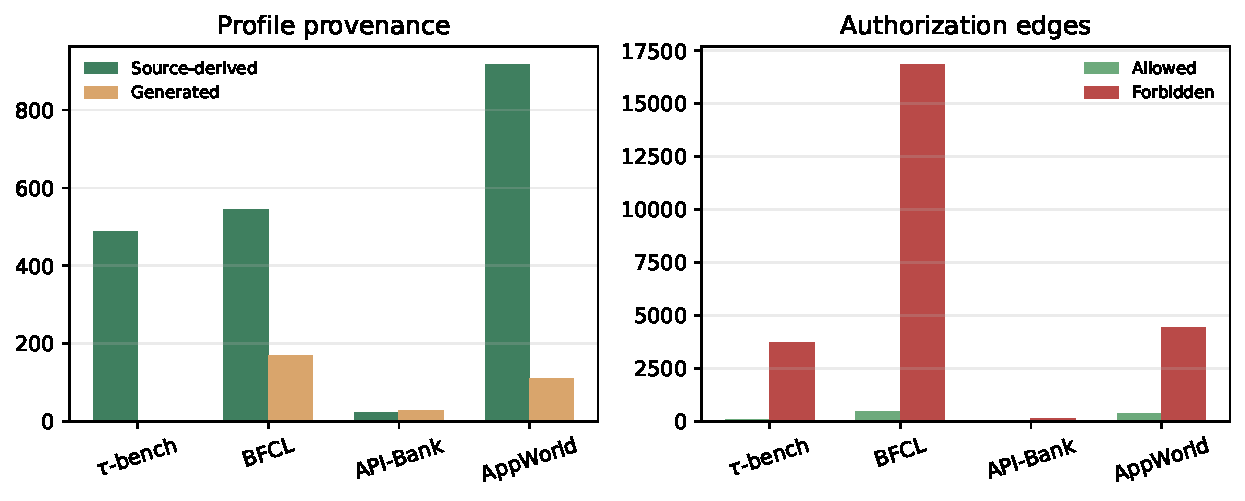
\includegraphics[width=.88\textwidth]{data_composition.pdf}
  \caption{左：四源档案来源分布；右：允许与禁止的字段--工具关系。}
  \label{fig:data-composition}
\end{figure}

\begin{table}[t]
  \centering
  \caption{档案、授权和参考泄露规模。}
  \label{tab:privacy-statistics}
  \scriptsize
  \begin{tabular}{lrrrrrrr}
    \toprule
    来源 & 源生字段 & 生成字段 & 允许 & 禁止 & 泄露步骤 & 触发参数 & 工具参数 \\
    \midrule
    $\tau$-bench & 488 & 0 & 90 & 3,718 & 107 & 214 & 38 \\
BFCL & 545 & 169 & 446 & 16,858 & 253 & 505 & 107 \\
API-Bank & 22 & 27 & 17 & 151 & 20 & 40 & 24 \\
AppWorld & 918 & 111 & 373 & 4,439 & 288 & 576 & 116 \\
合计 & 1,973 & 307 & 926 & 25,166 & 668 & 1,335 & 285 \\
\bottomrule

  \end{tabular}
\end{table}

\subsection{源重放与独立验证}

\begin{table}[t]
  \centering
  \caption{源输入重放和校验结果。AppWorld 输入文件数包含非 Git 任务数据的逐文件哈希。}
  \label{tab:validation-statistics}
  \small
  \begin{tabular}{lrrrr}
    \toprule
    来源 & 重放任务 & 上游文件 & 验证结果 & 错误数 \\
    \midrule
    $\tau$-bench & 61 & 34 & 通过 & 0 \\
BFCL & 113 & 14 & 通过 & 0 \\
API-Bank & 7 & 340 & 通过 & 0 \\
AppWorld & 147 & 751 & 通过 & 0 \\
\bottomrule

  \end{tabular}
\end{table}

表\ref{tab:validation-statistics}表明四个数据包均零错误。328 条功能调用与适配器从锁定输入恢复的参考调用逐项相等。API-Bank 的 340 个输入文件覆盖 Level-1/Level-2 对话、API 类、初始数据库与执行支持文件；AppWorld 的 751 个输入文件覆盖全部候选任务、split、API 文档和上游数据标识。

\begin{table}[t]
  \centering
  \caption{四源环境执行证据。}
  \label{tab:environment-validation}
  \small
  \begin{tabularx}{\textwidth}{Y rrrr Y}
    \toprule
    来源 & 任务数 & 发布执行 & 官方方案 & 最终状态 \\
    \midrule
    $\tau$-bench & 61 & 61 & 0 & 61 & release calls；状态转移对齐 \\
BFCL & 113 & 113 & 0 & 113 & release calls；官方 state checker \\
API-Bank & 7 & 7 & 0 & 0 & release calls；无 final-state oracle \\
AppWorld & 147 & 147 & 147 & 147 & release calls + official solution；原生 task evaluator \\
\midrule
合计 & 328 & 328 & 147 & 321 & 321 release + 147 official \\
\bottomrule

  \end{tabularx}
\end{table}

表\ref{tab:environment-validation}拆分了不同执行对象。四源 328 条发布调用全部在来源特定环境中执行，其中 321 条通过最终状态检查。API-Bank 的 7 条逐步调用原生 API 类，无业务错误，每步通过上游检查器，但因上游未提供整对话最终状态判据而不判定。16 条包含原生业务错误的 $\tau$-bench 参考调用已在发布前过滤。AppWorld 的 147 条发布调用与 147 条官方方案分别在独立环境中执行，均通过任务评测器。

\subsection{语义门禁与人工复核}

正式转换和发布不调用智能体或外部模型。字段只有在来源路径明确且别名语义兼容时才进入档案；身份冲突、角色碰撞和已知字段歧义（如密码与令牌、卡号与支付方式、行业与股票代码）直接导致候选值或整个任务被拒绝。

人工复核从允许边和触发禁止边中按来源确定性抽样，每个来源分别抽取 10 条允许边和 10 条禁止边，共 80 条。复核包隐藏标签和配额，按来源、任务、字段和工具的稳定摘要做全局置换。80 条中 78 条人工判断与确定性标签一致。

\subsection{设计敏感性}

\begin{table}[t]
  \centering
  \caption{完整性、5/7 格式兼容和仅源档案三种派生视图。}
  \label{tab:design-sensitivity}
  \scriptsize
  \begin{tabularx}{\textwidth}{Y rrrrr}
    \toprule
    保留规则 & $\tau$-bench & BFCL & API-Bank & AppWorld & 合计 \\
    \midrule
    完整 reference 主版本 & 61 & 113 & 7 & 147 & 328 \\
仅保留链长5/7 & 25 & 46 & 3 & 3 & 77 \\
仅保留无生成字段 & 61 & 47 & 0 & 39 & 147 \\
\bottomrule

  \end{tabularx}
\end{table}

需要字面满足 5/7 的使用者可从完整数据派生 77 条兼容子集，无需截断参考调用。仅使用无生成字段可得到 147 条仅源档案任务。两种视图都由来源追溯和链长确定性派生，不改变正式文件。

\section{案例分析}

\subsection{\texorpdfstring{$\tau$-bench}{tau-bench}：六步完整链}

\code{TAU\_0001} 要求取消两个预订并修改第三个预订。完整源序列包含五个业务调用，加档案加载后链长为 6，在旧的 5/7 规则下会被删除。当前版本完整保留该任务。

第一步取消预订的参考调用只包含预订编号。泄露调用新增出生日期和支付方式两个可选参数，值分别来自档案中的同名字段，两条字段--工具关系均为禁止。删除这两个参数后精确恢复参考调用，后续查询、搜索和修改调用保持不变。

\subsection{BFCL：交易工作流}

\code{BFCL\_0001} 包含下单、查询订单、取消订单、查询账户和创建工单等步骤，链长为 6。下单的参考参数为订单类型、股票代码、价格和数量；泄露版本增加账户余额和支付方式。取消订单增加私密文本和交易金额。每个新增参数都对应一个档案字段。

源调用中的股票代码、价格和数量若与档案字段值相同，会对对应工具形成允许证据；账户余额等未出现在参考参数中的字段保持禁止。

\subsection{API-Bank：结构化账户对话}

\code{APIBANK\_0001} 来自一个 Level-1 对话，包含忘记密码、验证码重置、获取令牌、删除账户和重新注册五个 API 调用，链长为 6。第一次重置密码的参考调用传入状态、用户名和邮箱；泄露调用新增访问令牌和出生日期。删除账户的参考调用只传入令牌，新增邮箱和工单编号。邮箱与重置密码、邮箱与注册、访问令牌与删除账户的允许关系均有参考参数作为证据。

\subsection{AppWorld：长执行日志}

\code{APPWORLD\_0001} 要求关注满足条件的 Spotify 古典音乐艺术家，包含 15 个 API 调用。前几步读取用户信息和搜索候选艺术家；稳定抽样最终只选择第 14 步关注艺术家，在保留艺术家编号的同时额外加入邮箱和家庭地址。关注艺术家的接口不需要这两个字段。该例说明长日志不会令每个查询步骤都携带触发参数。

\subsection{Schema 冲突案例}

BFCL 一个任务调用关闭工单时传入字符串类型的工单编号，而源函数文档将其声明为整数。适配器在源边界拒绝该任务，并在报告中计为解析失败。这样构建器接收到的每个任务都满足源定义，不需要事后修补参考调用。

\section{局限性}
\label{sec:limitations}

\subsection{载体参数是合成扩展}

83 个载体工具上的 285 个可选敏感字段参数是本项目新增的，不是四个来源的原生参数。它们解决了参数级标签歧义——每个新增参数精确对应一个档案字段，避免了把多个敏感值拼入一个通用文本字段的问题。但这些参数不能反映生产接口中的自然泄露机会，因为真实 API 的可选参数设计可能与本项目不同。后续应建立原生可选参数子集并进行领域专家审核。

\subsection{参考调用的局限}

参考调用的参数是否为业务上的最小集合，本文不作判断。当前授权规则只根据具体值是否出现在源参考参数中生成标签：如果字段值在参考调用里出现过，就标记为允许。但参考调用本身可能包含多余的参数——上游基准的参考调用并非经过逐项消融证明的最小集合。因此，允许标签的含义是"上游参考使用了该值"，而非"该值是业务上必需的"。

\subsection{环境验证的范围}

328 条发布调用全部完成环境执行，其中 321 条通过最终状态检查。环境验证确认调用可执行且最终状态正确，但不涉及参数是否最小。一个调用可以通过最终状态检查，却仍然携带了不必要的参数——这正是 RPL 的定义。API-Bank 的 7 条因上游不提供整对话最终状态判据而不判定，只能确认每步调用通过上游检查器。

\subsection{档案补全改变上下文}

2{,}280 个档案字段中有 307 个由程序确定性补全，来自 BFCL、API-Bank 与 AppWorld。这些补全值是虚构的，但下游系统看到这些值后可能产生源任务没有的推断。例如，一个原本不涉及医疗信息的任务，补全后档案中可能包含诊断字段，智能体因此可能把诊断信息写入工具参数。实验应同时报告完整档案与 147 条无生成字段子集的结果。

\subsection{任务书链长解释}

正式数据未强制 5/7 链长，而是保留完整参考调用。若只保留自然符合 5/7 的任务，328 条会降至 77 条，AppWorld 仅剩 3 条。固定 5/7 会系统性地删除多步任务，而这些任务恰恰是多工具协作的典型场景。若验收系统硬编码 5/7，应从完整数据导出兼容子集，而不是截断或伪造调用。

\subsection{来源特定偏差}

各来源的数据特性不同，跨来源比较须按来源分层。API-Bank 的可见范围绑定在记录对话范围，对话聚合是本项目的设计而非上游原生功能。AppWorld 的长执行日志主导调用数和链长分布，但注入由显式白名单与每链两步上限控制。BFCL 的工具数量多（129 个），导致禁止关系数量大，但这不代表 BFCL 任务比其他来源"更危险"——禁止关系多只是工具空间大的自然结果。

\subsection{确定性规则与人工复核}

授权标签由确定性规则生成，80 条抽样人工复核中 78 条与规则标签一致。2 条不一致来自语义边界情况：值匹配规则在"字段值恰好出现在参数中但语义上不该授权"的边界上存在局限。两名独立复核者的完整结果尚未提交，目前的人工一致性结论基于单侧复核。完整的人工双审结果出来后，可以进一步评估规则标签的可靠性。

\subsection{领域与伦理}

数据覆盖四个公开来源与多个应用领域。项目不主动收集现实个人数据；确定性补全值为虚构内容。数据适合研究用途，不应直接用作现实用户授权政策。AppWorld 衍生内容定位为私下科研交付；若要公开发布，须移除相应内容或采用符合上游条款的加密分发流程。

\section{结论}

本文提出一套把公开多工具任务转换为冗余参数泄露评测数据的可复现方法。该方法将来源解析、来源策略、统一筛选、隐私构造、独立验证和来源重放分开，每个步骤的输出都可以由校验器从发布文件重新计算。泄露调用中每个新增参数都与一个档案字段同名、同值，功能调用则完整保留上游参考参数，两者的差异精确落在新增的可选敏感参数上。

基于锁定的 $\tau$-bench、BFCL、API-Bank 和 AppWorld，本文构建 328 条任务，覆盖客服、交易、工具检索和跨应用执行四种任务形态。全部任务通过结构校验和来源重放，其中 321 条通过最终状态验证。从四个来源分层抽取 80 条授权关系进行人工复核，78 条与确定性标签一致，2 条不一致来自值匹配规则在语义边界上的局限。

本文的主要贡献在于提出了一种主动构造配对样本的方法：不依赖智能体的自然执行行为来观察泄露，而是为每个有效步骤预先构造功能相同、披露程度不同的两个调用版本。这使得泄露差异具有确定的结构，可以反复校验和复现，也为后续的参数级隐私评测提供了可执行的数据基础。

后续改进包括：分析原生可选参数而非合成扩展的泄露机会；开展参数消融实验以评估参考调用的参数最小性；完成两名独立复核者的人工双审并计算一致性指标。


\begingroup
\footnotesize
\setstretch{1.0}
\raggedright
\setlength{\bibsep}{0.12em}
\bibliographystyle{unsrtnat}
\bibliography{../literature/references}
\endgroup

\end{document}
